\documentclass[tikz]{standalone}

\usepackage{amsmath}

\renewcommand{\vec}[1]{\boldsymbol{#1}}

\tikzset{>=latex}
\begin{document}
\begin{tikzpicture}
  \node[coordinate] (A) at (4.8,3.9) {};
  \node[coordinate] (F) at (13,1.5) {};
  \node[coordinate] (Q) at (10.5,1.9) {};
  
  \node[coordinate] (fa_final) at (3.45,4.8518) {};
  \node[coordinate] (ma_final) at (5.55,6.56) {};

  \node[coordinate] (r_final) at (11.7,2.5) {};
  
  \node[anchor=south west,inner sep=0] at (0,0) {
    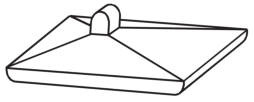
\includegraphics[width=\textwidth]{fri_figure}};

  \node[left=5, below=1, font=\sffamily] at (A) {\Large A};
  \node[below=3, font=\sffamily] at (Q) {\Large Q$^*$};
  \node[right=8, above=1, font=\sffamily] at (F) {\Large F};

  \draw[->=stealth, very thick,line width=1mm, red] (Q) -- (F);
  
  \draw[black, fill=red] (A) circle (5pt);
  \draw[black, fill=red] (F) circle (5pt);
  \draw[black, fill=red] (Q) circle (5pt);
  

  \draw[->=stealth, very thick, line width=1mm, black]  (A) -- (fa_final) node[font=\sffamily, left=7, above=2] {\Large $-\vec{F}_A$};
  \draw[->=stealth, very thick, line width=1mm, orange]  (A) -- (ma_final) node[font=\sffamily, right=7, below=20] {\Large $\vec{M}_A$};
  \draw[->=stealth, very thick, line width=1mm, black]  (F) -- (r_final) node[font=\sffamily, right=10] {\Large $\vec{R}$};
\end{tikzpicture}
\end{document}
